
%(BEGIN_QUESTION)
% Copyright 2006, Tony R. Kuphaldt, released under the Creative Commons Attribution License (v 1.0)
% This means you may do almost anything with this work of mine, so long as you give me proper credit

Energy is required to compress or stretch a mechanical spring, because there is a force exerted over a parallel distance.  Calculating the work done in compressing or stretching a spring is more complicated than calculating work done when lifting a weight, because the force ($F$) is not constant.  Most springs exhibit a linear relationship between force and displacement (distance compressed or stretched) over short distances which is known as {\it Hooke's Law}:

$$F = kx$$

\noindent
Where,

$F$ = Force required to compress or stretch a spring by $x$ amount, in pounds (lb), or Newtons (N)

$x$ = Distance that the spring is compressed or stretched, in feet (ft), or meters (m)

$k$ = Constant of the spring, in pounds per foot (lb/ft), or Newtons per meter (N/m)

\vskip 10pt

Spring-operated weight scales exploit this principle of linearity: doubling the weight applied to a spring scale doubles the motion of the needle as it registers weight on a linear scale.

To calculate the amount of {\it work} done in compressing or stretching a spring, we must somehow account for the fact that force is {\it not} constant as the spring deforms.  Here, graphing force versus displacement is a helpful tool for calculating work.

Graph the force required to compress a spring with a constant of 60 pounds per foot, then calculate the amount of work required to compress it 3 feet:

$$\includegraphics[width=15.5cm]{i01575x01.eps}$$

\vskip 20pt \vbox{\hrule \hbox{\strut \vrule{} {\bf Suggestions for Socratic discussion} \vrule} \hrule}

\begin{itemize}
\item{} At which end of the spring's motion (0 feet of stretch, or 3 feet of stretch) does the spring store the most energy {\it per inch} of additional stretch? 
\item{} If you were to plot a graph of stored energy per inch of spring motion, what shape would that graph exhibit?
\item{} Identify the mathematical sign (positive or negative) of force ($F$), differentials of distance ($dx$), and work ($W$) while the spring is being {\it loaded} by an external force.
\item{} Identify the mathematical sign (positive or negative) of force ($F$), differentials of distance ($dx$), and work ($W$) while the spring is being {\it unloaded} towards its relaxed state.
\item{} Suppose this spring resided inside of an air-to-open pneumatic control valve.  If the control loop is oscillating -- thus making the valve's stem move up and down periodically -- what does the calculated work of spring compression represent in terms of compressed air consumption?  Would this quantity of work be significant in any way to us, or is it academic?
\item{} Suppose an air-to-open pneumatic control valve is cycling $\pm$10\% near the fully-shut position.  Now suppose that same valve is cycling $\pm$10\% near the fully-open position.  In which condition does the control valve consume the greatest rate of compressed air?  Explain why.
\end{itemize}

\underbar{file i01575}
%(END_QUESTION)





%(BEGIN_ANSWER)

$$\includegraphics[width=15.5cm]{i01575x02.eps}$$

%(END_ANSWER)





%(BEGIN_NOTES)

Remember that the area of a triangle is base times height divided by 2.

\vskip 10pt

We may also solve this problem if we know how a bit of calculus:

$$W = \int_0^3 F \> dx \hbox{\hskip 50pt} F = kx$$

$$W = \int_0^3 kx \> dx$$

$$W = \int_0^3 60x \> dx$$

$$W = 60 \int_0^3 x \> dx$$

$$W = 60 \left[ {1 \over 2}x^2 \right]_0^3$$

$$W = 60 \left[ {3^2 \over 2} - {0^2 \over 2} \right]$$

$$W = 60 \left[ 4.5 - 0 \right]$$

$$W = 60 \left[ 4.5 \right]$$

$$W = 270 \hbox{ ft} \cdot \hbox{lb}$$

%INDEX% Mathematics, calculus: integral (work)

%(END_NOTES)


